\documentclass[herrin-thesis.tex]{subfiles}
\begin{document}
\section{Motivation}
Ideally, EXO-200 would only trigger on events that are due to particles interacting in the liquid xenon. Unlike the detectors at hadron colliders that have a large event rate and must selectively trigger, EXO-200 only sees about one event every 10 seconds. Therefore, the triggers do not need to be sophisticated, and indeed err on the side of including events that may not be interesting.

These simple triggers, however, allow events that are not actually due to interactions in the detector to make it into the data. One common source of spurious events is noise, for example due to microphonic vibration of the signal readout cables due to loud noises. When these noise signals go through processing, they can slow down the processing due to odd signal shapes and large multiplicity. Furthermore, they can masquerade as signals. As described below, one of the most common types of noise can be tagged as a TPC muon. These noise events are frequent enough that the deadtime enforced after a TPC muon would cause a significant hit to live time. And so code was developed to identify and tag noise events.

\section{Types of Noise Events}
\subsection{Unphysically Negative Signals on the Collection Wires}
The collection wires normally collect drifting ionization, which produces a positive-going signal. Some collection wire channels may show a small negative-going induction signal when a signal is collected on a neighboring channel. However, there should not be events in which a large number of collection wire channels have a negative signal without being preceded by or simultaneous to a positive signal.

These events are identified by summing all collection wire waveforms. The baseline of this sum is taken by averaging the first 256 samples of the waveform. If the sum waveform drops 270 ADC counts below baseline before any individual wire goes above 30 ADC counts, the event is tagged as noise.

\begin{figure}[tbp]
\centering
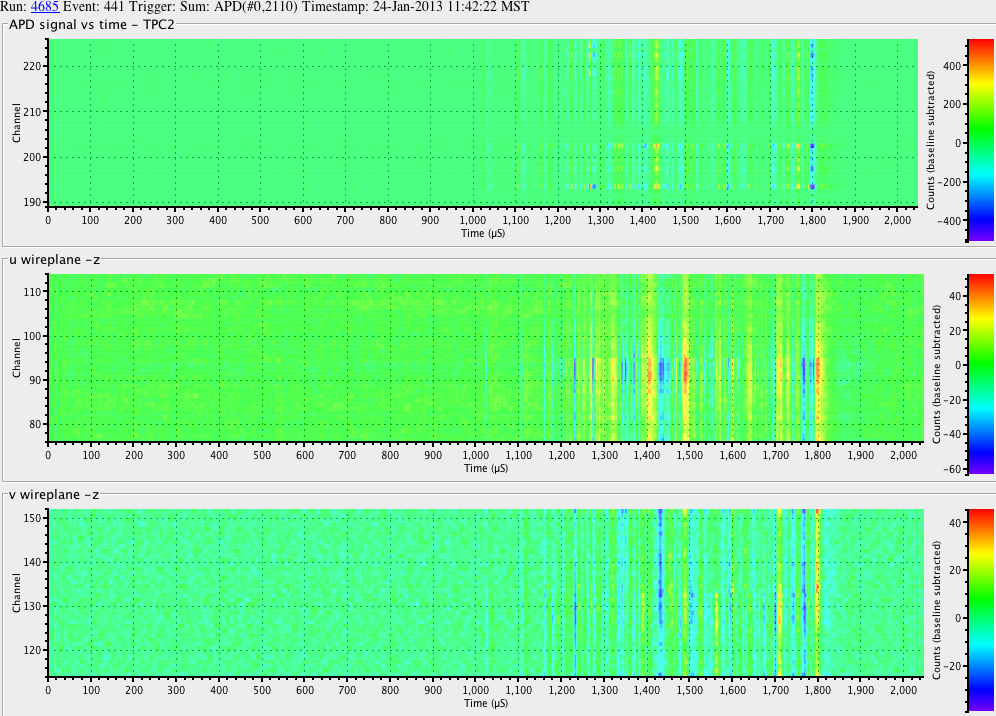
\includegraphics[width=\columnwidth]{./plots/noise_eventdisplay_run_4685_ev_0441.png}
\caption[Collection wires negative noise]{A noise event which shows the collection \((u)\) wires going unphysically negative before any individual wire shows a psoitive signal.}
\label{fig:noise_sum_u_neg}
\end{figure}

\Cref{fig:noise_sum_u_neg} shows an example of a typical event caught by this check. These events would otherwise be problematic for the muon tagging algorithm (\cref{ch:muons}) because they exhibit lines of positive collection signals and negative inductions signals that resemble a muon passing parallel to the wire plane.

\subsection{``Glitch'' events}
For a period of time, the high-voltage supply for the EXO-200 cathode would occasionally cause a large number of channels in the TPC to complete saturate. The exact origin of these ``glitch'' events is still unknown. They seem to be electronic, since they still saturated channels when the APD gains were reduced to unity.

These events are identified by looking for more than 100 channels completely saturated.

\begin{figure}[tbp]
\centering
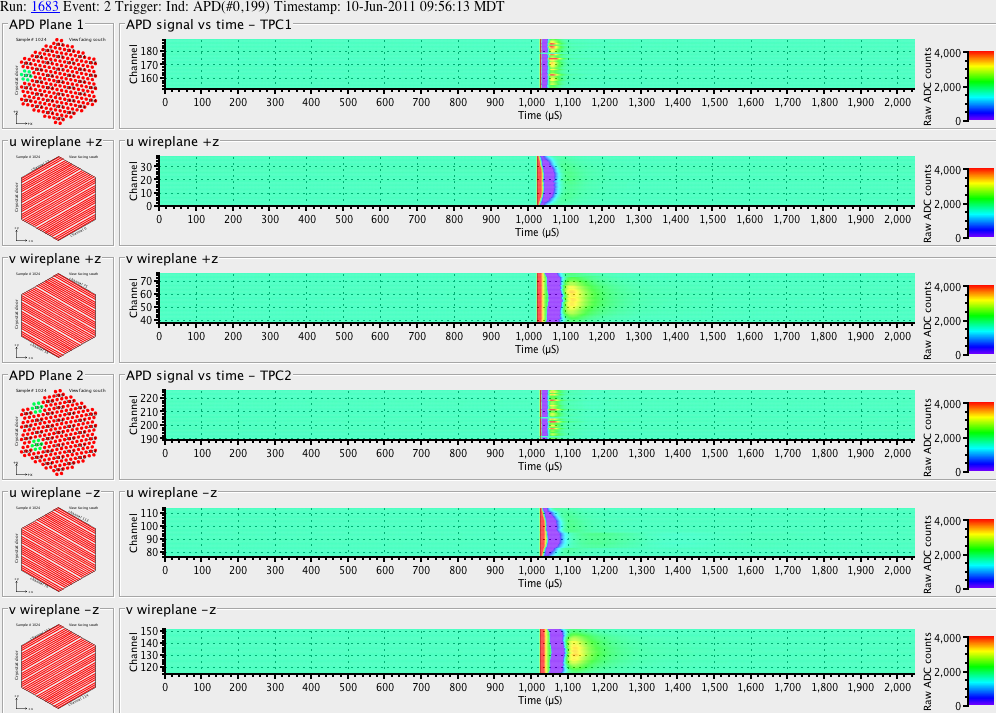
\includegraphics[width=\columnwidth]{./plots/noise_eventdisplay_run_1683_ev_0002.png}
\caption[``Glitch'' noise]{An example of a ``glitch'' event showing a large number of saturated channels.}
\label{fig:noise_glitch}
\end{figure}

\Cref{fig:noise_glitch} shows an example of a ``glitch'' event. The only other type of event that saturates a large number of channels are high-energy TPC muons, or  muons stopping and decaying in the TPC. However, these are rare, and so this noise check only slightly reduces the efficiency of muon tagging.

\subsection{APD ``bouncing'' events}
In some events, the APD signals seem to spontaneously saturate, go far below their baseline, rebound, and then bounce below or high above the baseline again. This seems to be accompanied by noise in the muon veto system, though it has proven difficult to diagnose.

These events are identified by looking for any APD channels that saturate, then fall below 20 ADC counts absolute (without considering baseline), recovering to above 1024 ADC counts (again absolute, which is 1/4 full scale), and then either dipping back below 1024 ADC counts or bouncing above 2048 ADC counts (typical baselines are \(\sim\)1600 ADC counts). 

\begin{figure}[tbp]
\centering
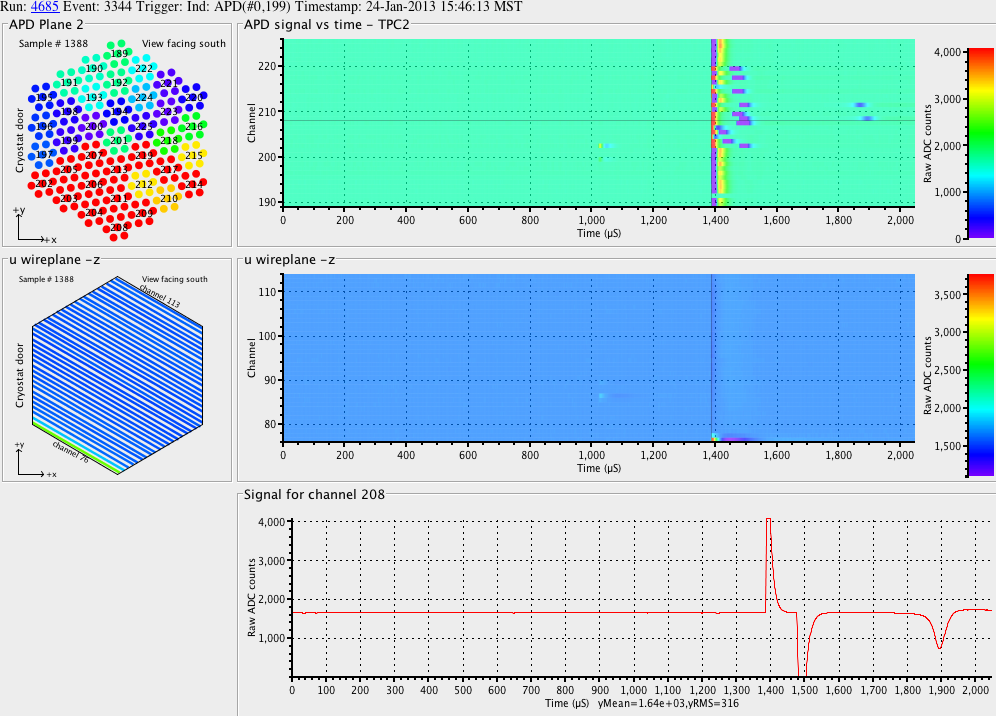
\includegraphics[width=\columnwidth]{./plots/noise_eventdisplay_run_4685_ev_3344.png}
\caption[APD ``bouncing'' noise]{A noise event with an APD channel signal ``bouncing''.}
\label{fig:noise_apd_bounce}
\end{figure}

\Cref{fig:noise_apd_bounce} shows an example of this type of noise. This noise events could otherwise be tagged as muons, since the signal often bleeds over into the wire signals.

\end{document}